

\section*{Q.2b. \emph{Polygonization over a hole} (\ph)}
Lets denote the problem as  \emph{Polygonization over a hole} (\ph). We label a point as \emph{Red} or \emph{Blue} based on whether it belongs to the set to be polygonized or to the hole (lets denote cardinality of these sets by $r$ and $b$ respectively and $n=r+b$). We consider the following assumptions:
\begin{multicols}{2}
	\begin{itemize}
%		\item If the hole polygon is spiral then it has constant number of bends.
		\item All points have integral, general coordinates.
		\item No red point lies inside \HH.
		\item Every pair of blue points has a finite distance between them (used to find a point infinitesimaly away from each blue point).
	\end{itemize}
\end{multicols}
A trivial necessary (not sufficient) condition for the instance to be a Yes Instance is that the convex hull of red points completely contains \HH inside it. In case a such a convex hull doesn't exist, we can always deal it by adding $3$- extra red points in the form of a triangle which contains all the red and blue points (imagine a large such triangle). W.l.o.g from now on we will implicitly assume that such a convex hull exists. Although it should be noted that this is not a sufficient condition as there may be points trapped inside \HH (if it is spiral) not "visible" to the convex hull.


We now realize the problem from a graph theoretic view. We compute a (simple, undirected) visibility graph \GG as follows: Vertices are Red Points. There is an edge between two nodes iff they are visible to each other (i.e. the line segment joining the two given points has no intersection with the hole). This takes $O(n^2)$ time and space. It is evident that there is a planar hamiltonian cycle in \GG if there is a polygonization of the points (we need it to planar to ensure that the polygon is simple and no-edges are crossing each other).
Again, this condition alone is not sufficient as the ham-cycle may output a polygon with the \HH completely outside it (as shown in \Cref{fig:hamcycle}.


However combining the above two conditions satisfies the sufficiency. This can be intuitively observed from the fact that a case like \Cref{fig:hamcycle} cannot exist if the convex hull of red points encloses the hole. This gives us the necessary and sufficient conditions for a the given \ph instance to be a Yes Instance:
\begin{enumerate}
	\item $\exists$ a planar hamiltonian cycle in visibility graph \GG of input instance.
	\item The convex hull of red points must be enclosing \HH
\end{enumerate}

However we realise that finding a Ham-Cycle which is planar (note that it is not same as Planar-HamCycle Problem) is \NPH, implying that we need exponential time to solve the problem (enumerate all possible vertex orderings and check if they form a planar HamCycle : $O^*(n^n)$).

Now assuming that we have the fraternity to add linear number of additional points to the red set. For every blue vertex we add a point infinitesimally close to it and outside of \HH (this can be done by considering exterior angle bisector and placing point on it at a some $\eps$ distance away). This adds almost $b$ extra points. Lets label this new set of points as gray. Intuitively, we do this to handle the case when there are points not connected to (visible to) points of convex hull. Adding the gray points ensures that every point can be connected (using a disjoint subset of gray points) to the convex hull (consider it as an envelop over the hole which acts as an escape route for the hidden points). 

[Enveloping Algorithm] More formally, to find \PP, we start with choosing two gray points corresponding to an edge of \HH). For these two points, find the maximal simple-polygonal chain of red points; disjoint from the area of the hole; starting and ending at these two points. Then we consider the next pair of gray points (corresponding to the adjoining edge of previously considered edge) and form a similar simple-polygonal chain. We halt at the point when all edges have been considered. (its analogous to a walk around the hole \HH, iteratively building the chain to find \PP). This completes the description of algorithm. 

[Complexity] We first do a simple pre-processing in time $O(n^2)$ as done in visibility graph. Then at each step of iterative algorithm, we have to check all other points and their visibilities (searching the adjacency matrix of \GG) which will again take $O(n^2)$ time. Summing up over all iterations, time complexity comes out to be $O(b.n^2)$. (Please note that adding $b$ gray vertices, changes $n$ from $(r+b)$ to $(r+2b)$, and thus doesn't change n (asymptotically)).


\begin{figure}[!h]
	\centering
	\subfigure[A Counter Example where visibility graph has a planar ham-cycle but \ph is a NO instance.]{
		\resizebox{!}{5cm}{
			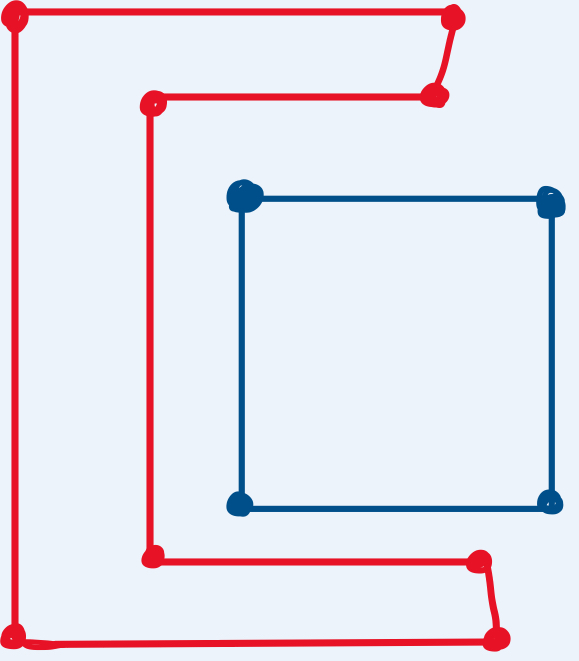
\includegraphics[scale=.1]{hamcycle.jpg}
			\label{fig:hamcycle}
		}
	}\hspace{2cm}
	\subfigure[A run of Enveloping algorithm. Green color decribes the envelop formed by algorithm. Other vertices are colored as per convention.]{
		\resizebox{!}{5cm}{
			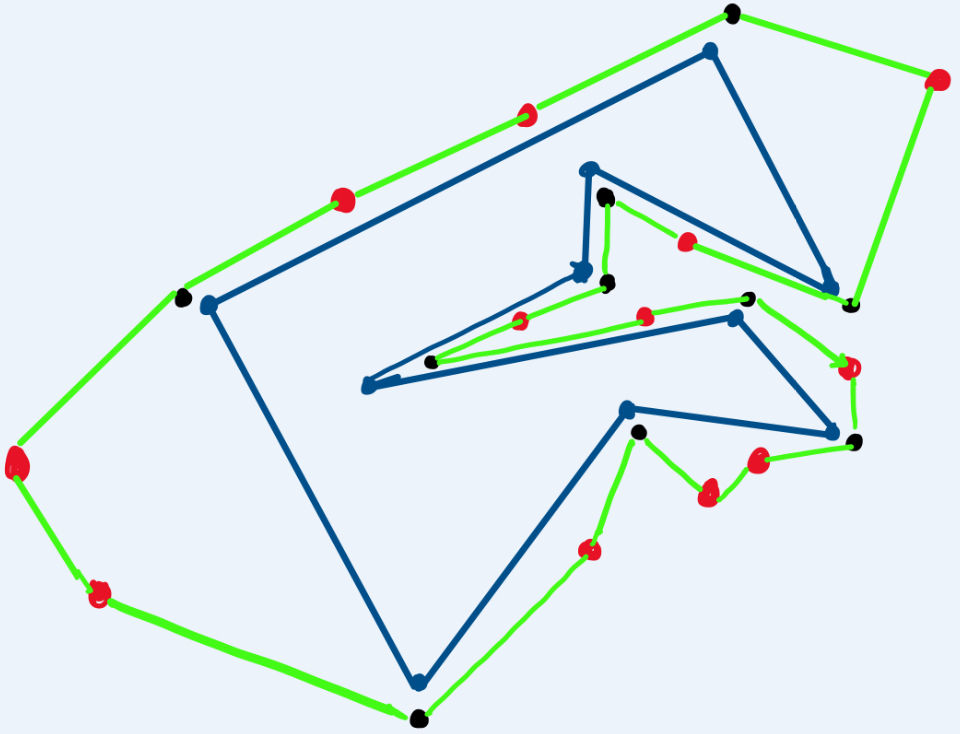
\includegraphics[scale=.1]{walk.jpg}
			\label{fig:walk}
		}
	}
	\label{fig:gen}
\end{figure}


